\documentclass[11pt]{article}
\usepackage[a4paper,margin=2.4cm]{geometry}
\usepackage{booktabs,graphicx,amsmath,hyperref,xcolor}
\hypersetup{colorlinks,linkcolor=blue!50!black,citecolor=blue!50!black,urlcolor=blue!50!black}
\usepackage[numbers,sort&compress]{natbib}

\title{A Radiograph Foundation Model Did Not Transfer Better Than a Generic One:\\
\large A Pre-Registered Linear-Probe Comparison for Knee Osteoarthritis Grading}
\author{Mithil Nagabathula\\University of East London\\\texttt{mithilnishu2000@gmail.com}}
\date{October 2026}

\begin{document}
\maketitle

\begin{abstract}
Choosing a backbone is the first decision in building an imaging model, and domain-specific foundation models are an attractive
default. We report a pre-registered gate experiment from KneeScope, a research prototype for Kellgren--Lawrence (KL) grading of
knee radiographs, together with follow-up analyses. Three frozen backbones were compared with identical linear probes on 8{,}260
knee radiographs from 4{,}130 Osteoarthritis Initiative participants, under a leakage-audited patient-level split, with the test split
kept sealed. RAD-DINO, pretrained on chest radiographs, reached a quadratic weighted kappa (QWK) of 0.629, not distinguishable from an
ImageNet ResNet-50 (0.602; paired difference +0.027, 95\% CI \([-0.023, 0.073]\)). DINOv2 ViT-B, pretrained on natural images,
reached 0.686, better than both ImageNet (+0.084, \([0.040, 0.127]\)) and RAD-DINO (+0.057, \([0.012, 0.100]\)). The pre-registered
rule therefore switched the project to DINOv2. Follow-up analyses showed the advantage at every training-set size: with a quarter of
the training images DINOv2 matched RAD-DINO trained on all of them, and concatenating the two backbones added nothing. Every probe
failed on the doubtful grade (KL1 recall 0.11--0.19). Errors on a patient's two knees were correlated, which makes patient-level
resampling necessary for honest confidence intervals. A radiography label on a foundation model is not evidence that it suits a new
anatomy; a cheap frozen-probe gate is.
\end{abstract}

\section{Introduction}
Knee osteoarthritis severity is graded on radiographs with the Kellgren--Lawrence scale \cite{kellgren1957}, from 0 (none) through 1
(doubtful) to 4 (severe). Deep networks have graded KL from Osteoarthritis Initiative (OAI) images for a decade
\cite{antony2016,tiulpin2018,chen2019knee}. Self-supervised foundation models now offer strong frozen features: DINOv2 trained on 142
million natural images \cite{oquab2024dinov2} and RAD-DINO trained on chest radiographs \cite{perezgarcia2025raddino}.

KneeScope is a research prototype, explicitly not a medical device, that grades KL with a parameter-efficient (LoRA \cite{hu2022lora})
adaptation of a foundation backbone. Its design initially chose RAD-DINO on the argument that radiograph pretraining should transfer to
other radiographs. That argument was untested: chest and knee radiographs differ in anatomy, texture and the features that matter. The
project therefore pre-registered \cite{nosek2018prereg} a gate experiment, C0, with a fixed decision rule, before any fine-tuning.
This paper reports C0 and extends it with analyses on the same frozen features.

\section{Methods}
\paragraph{Data.} The OAI-derived knee KL dataset of Chen \cite{chen2018data,chen2019knee}: 8{,}260 single-knee radiographs at
\(224\times224\) pixels from 4{,}130 participants (both knees, one visit each) \cite{oai}. KL distribution: 39\% grade 0, 18\% grade 1,
26\% grade 2, 13\% grade 3, 3\% grade 4. KneeScope re-split the data by patient into training (4{,}952 images, 2{,}476 patients),
calibration (828), validation (826, 413 patients) and test (1{,}654). A leakage audit enforced seven properties (patient disjointness,
both knees of a patient in one split, exact and perceptual near-duplicate containment, file-name identity, a pinned test-set hash, and
complete assignment); all passed. No model has been evaluated on the test split.

\paragraph{Backbones and features.} Three frozen backbones: ImageNet ResNet-50 \cite{he2016resnet} as the reference, RAD-DINO
\cite{perezgarcia2025raddino}, and DINOv2 ViT-B/14 \cite{oquab2024dinov2}. Each image is represented by the concatenation of the class
token and the mean of the patch tokens (pooled feature maps for the CNN), giving 1{,}536 dimensions for the ViTs and 4{,}096 for
ResNet-50. Features were extracted once on the author's machine and cached with hashes of the data manifest and split.

\paragraph{Probe and decision rule.} Standardised features feed a multinomial logistic regression with inverse regularisation \(C\)
from \(\{10^{-3},\dots,10\}\). The primary metric is QWK \cite{cohen1968kappa}. The pre-registered rule compared RAD-DINO with ImageNet:
keep RAD-DINO if \(\Delta\mathrm{QWK}\geq 0.03\); switch away if it is clearly worse (\(\Delta<0\) with a CI entirely below 0); otherwise
evaluate the pre-registered fallback, DINOv2. Confidence intervals are 95\% bootstrap intervals that resample patients (both knees
together); differences use a paired bootstrap on the same patients.

\paragraph{Follow-up analyses.} (1) A stricter choice of \(C\) by 5-fold patient-grouped cross-validation on the training split, since
C0 selected \(C\) on validation. (2) Label efficiency: probes trained on 1--100\% of training patients, five random draws per size.
(3) Fusion of DINOv2 and RAD-DINO features. (4) Calibration (expected calibration error, ECE \cite{guo2017calibration}) and selective
prediction (area under the risk--coverage curve, AURC \cite{geifman2017selective}). (5) The dependence between a patient's two knees.

\section{Results}
\begin{table*}[t]
\centering
\caption{Linear probes on frozen features, validation split (826 knees, 413 patients). Confidence intervals resample patients; $\Delta$ is a paired bootstrap against the ImageNet probe on the same patients. AURC is the area under the risk--coverage curve using the top-class probability (lower is better).}
\label{tab:main}
\footnotesize
\setlength{\tabcolsep}{3.5pt}
\begin{tabular}{lrrrrrr}
\toprule
Backbone & QWK [95\% CI] & $\Delta$ vs ImageNet & KL1 recall & KL0/1 AUROC & ECE & AURC \\
\midrule
ImageNet ResNet-50 & 0.602 [0.546, 0.654] & -- & 0.136 & 0.609 & 0.053 & 0.356 \\
RAD-DINO & 0.629 [0.577, 0.677] & +0.027 [-0.023, +0.073] & 0.110 & 0.647 & 0.085 & 0.356 \\
DINOv2 ViT-B & 0.686 [0.636, 0.732] & +0.084 [+0.040, +0.127] & 0.156 & 0.670 & 0.074 & 0.317 \\
DINOv2 + RAD-DINO & 0.682 [0.631, 0.724] & +0.080 [+0.037, +0.122] & 0.195 & 0.678 & 0.131 & 0.333 \\
\bottomrule
\end{tabular}
\end{table*}


\paragraph{The gate.} RAD-DINO's advantage over ImageNet (+0.027) fell short of the +0.03 threshold and its interval included zero, so
the rule returned its middle branch and the fallback was evaluated (Table~\ref{tab:main}). DINOv2's advantage over ImageNet (+0.084) had
an interval entirely above zero, and in a direct comparison DINOv2 also beat RAD-DINO (+0.057, 95\% CI \([0.012, 0.100]\)). The project
adopted DINOv2. Choosing \(C\) by cross-validation on the training split selected the same value as validation selection for every
backbone, so the C0 numbers did not depend on tuning against the evaluation split; our re-implementation reproduced C0's QWK to three
decimal places.

\paragraph{Label efficiency.} DINOv2 led at every training-set size (Figure~\ref{fig:label}, Table~\ref{tab:label}). With 1{,}238
images (25\% of patients) it reached 0.622, matching RAD-DINO and exceeding ImageNet trained on all 4{,}952. The gap was largest in
relative terms with very few labels: with 50 images DINOv2 reached 0.29 against 0.10--0.15 for the others.

\begin{figure}[t]
  \centering
  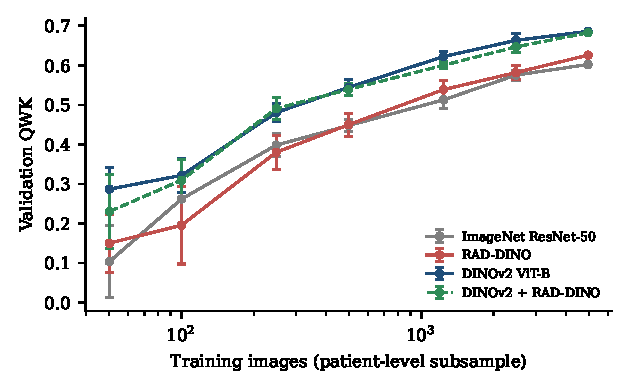
\includegraphics[width=0.62\linewidth]{figures/label_efficiency.pdf}
  \caption{Validation QWK of linear probes against the number of training images (mean \(\pm\) SD over five patient-level draws).}
  \label{fig:label}
\end{figure}

\begin{table}[t]
\centering
\caption{Mean validation QWK by training-set size (5 patient-level draws below 100\%).}
\label{tab:label}
\small
\setlength{\tabcolsep}{4pt}
\begin{tabular}{rrrrr}
\toprule
Training images & ImageNet & RAD-DINO & DINOv2 & Fusion \\
\midrule
50 & 0.104 & 0.150 & 0.287 & 0.230 \\
100 & 0.262 & 0.196 & 0.322 & 0.310 \\
248 & 0.398 & 0.380 & 0.481 & 0.491 \\
496 & 0.448 & 0.450 & 0.544 & 0.539 \\
1238 & 0.513 & 0.539 & 0.622 & 0.600 \\
2476 & 0.575 & 0.582 & 0.663 & 0.646 \\
4952 & 0.602 & 0.626 & 0.686 & 0.682 \\
\bottomrule
\end{tabular}
\end{table}


\paragraph{Fusion.} Concatenating RAD-DINO with DINOv2 did not improve on DINOv2 alone (0.683 against 0.686), and was worse calibrated
(ECE 0.131 against 0.074). RAD-DINO's features carried no complementary signal that a linear probe could use.

\paragraph{The doubtful grade.} All probes recalled KL1 poorly (0.11--0.19), and KL0-versus-KL1 discrimination was modest (AUROC
0.61--0.68). KL1 is the grade on which human readers disagree most, and frozen features with a linear head do not resolve it; this is the
part of the task that adaptation has to earn.

\paragraph{Calibration and selective prediction.} ECE ranged from 0.054 (ImageNet) to 0.085 (RAD-DINO). DINOv2 had the lowest AURC
(0.317), meaning its confidence ranked its own errors best: referring its least confident cases removed errors faster than for the other
probes.

\paragraph{Two knees per patient.} For the DINOv2 probe, an error on one knee raised the chance of an error on the other from 0.38 to
0.49 (\(\phi=0.11\)), and the two knees shared the same KL grade in 54\% of patients. Bootstrap intervals that resampled images were
11\% narrower than intervals that resampled patients (width 0.086 against 0.096): treating knees as independent overstates precision.

\section{Discussion}
The domain label on a foundation model was a poor guide. RAD-DINO's chest-radiograph pretraining did not transfer to knee grading better
than ImageNet features, while a generic self-supervised model trained on far more varied images did. A plausible reading is that knee KL
grading depends on joint-space narrowing, osteophytes and subchondral texture, which chest pretraining rarely exposes, whereas DINOv2's
scale and diversity give more transferable local features. We did not test this mechanism.

The methodological point is the more general one. The backbone choice was made on argument, then exposed to a cheap test with a decision
rule fixed in advance, and the rule overturned the argument. The test took one frozen forward pass per image and seconds of fitting on a
CPU. Projects that adopt a domain-specific foundation model by default can afford the same check.

\paragraph{Limitations.} Results are on the validation split of one dataset; the test split is sealed until the full model is trained,
and no external dataset was used. Images are \(224\times224\) crops, below RAD-DINO's native resolution of 518 pixels, which may
disadvantage it. A ConvNeXt arm was planned but not run. Linear probes measure frozen representations, not what LoRA adaptation will
reach. The dataset's grades come from OAI readings and inherit their inter-reader variability, which is largest at KL1.

\section{Conclusion}
In a pre-registered comparison, a chest-radiograph foundation model did not transfer to knee osteoarthritis grading better than ImageNet
features, while DINOv2 did, at every training-set size. Frozen-probe gates are cheap, and they can and should overturn a plausible
design choice before expensive fine-tuning begins.

\paragraph{Data and code.} The OAI-derived images are available from their original source \cite{chen2018data}; the extracted features
are not redistributed. Analysis code and result files will be released at
\newline\url{https://github.com/mithil2k2000-tech/kneescope-backbone-gate}.

\paragraph{Use of AI tools.} An AI assistant (Claude, Anthropic) helped write code for KneeScope and these analyses and draft text. The
author designed the project and the pre-registered rule, ran the feature extraction, reviewed all results and takes responsibility for
the content. KneeScope is a research prototype and not a medical device.

\bibliographystyle{plainnat}
\bibliography{refs}
\end{document}
